\documentclass{beamer}
\mode<presentation>
\usepackage[utf8]{inputenc}
\usepackage{graphicx}
\usepackage[english,italian]{babel} % se non fosse inglese dovrei indicare la lingua nella quale sillabare [Italian]
%\usepackage{fancybox}
\useoutertheme{}
\usepackage{beamerthemeshadow}
\usepackage{ulem}
\usepackage{courier}
\usepackage{tikz}
\usepackage{listings}
\usepackage{amsfonts}
\usepackage{fontawesome5}
\usepackage{color,soul}
\usetikzlibrary{snakes}
%\usepackage{beamertexpower}
%\beamertemplatetransparentcovereddynamicmedium
\usetheme{GTER} %(se vuoi mettere l'autore)
\useinnertheme{rectangles}
%\useoutertheme{infolines}
\usecolortheme[RGB={151,215,0}]{structure}
%\usecolortheme[RGB={0,99,29}]{palette quaternary}

\setbeamercovered{transparent}
\setbeamerfont{frametitle}{size=\small,series=\bfseries}
\setbeamercolor{frametitle}{bg=gter!}

\definecolor{lightred}{rgb}{0.94,0.04,0.04}
\definecolor{aqua}{rgb}{0.00,0.80,1.00}
\definecolor{lightgreen}{rgb}{0.01,0.40,0.03}
\definecolor{limegreen}{rgb}{0.61,1.00,0.10}
\definecolor{peach}{rgb}{1.01,0.85,0.72}
\definecolor{purple}{rgb}{0.93,0.51,0.93}
\definecolor{indianyellow}{rgb}{0.98,0.75,0.30}
\definecolor{brick}{rgb}{0.70,0.13,0.13}
\definecolor{springsteen}{rgb}{0.00,0.49,0.19}
%%%%%%%%%%%%%%%%%%%%%%%%%%%%%%%%%%%%%%%%%%%%%%%%%%%%%%%%%%%%%%%%%%%%%%
% \definecolor{gter}{rgb}{0.00,0.49,0.22} %verde GTER estratto da gimp
\definecolor{gter}{RGB}{151,215,0}
%%%%%%%%%%%%%%%%%%%%%%%%%%%%%%%%%%%%%%%%%%%%%%%%%%%%%%%%%%%%%%%%%%%%%%
\definecolor{lightorange}{rgb}{1.01,0.50,0.00}
\definecolor{royalblue}{rgb}{0.25,0.41,1.00}
\definecolor{lightgray}{rgb}{0.94,0.94,0.94}

% \definecolor{links}{HTML}{2A1B81}
\hypersetup{colorlinks,linkcolor=lightgray,urlcolor=springsteen}

% \title{Principi di cartografia numerica}
% \subtitle{I sistemi di riferimento}
% \author[]{Gter srl Innovazione in geomatica Gnss e Gis}
% %\author[]{Bianca Federici, Tiziano Cosso, \textbf{Roberto Marzocchi}, \\ Asimina Syriou}
% \author[]{Relatore: Manuele Pesenti}
% \date{Genova, settembre 2022}
% \logo{
\includegraphics[height=0.5 cm]{./Gter.png}}

\title{I dati vettoriali}
\subtitle{digitalizzazione, editing e gestione attributi}
\author[]{Gter srl Innovazione in Geomatica Gnss e Gis}
\author[]{Relatore: Manuele Pesenti}
\date{Genova, ottobre 2022} 
\logo{
\includegraphics[height=0.5 cm]{./Gter.png}}

\begin{document}
	{
		{
			\setbeamertemplate{footline}{} 
			\begin{frame}
				\titlepage
			\end{frame}
		}
		\addtocounter{framenumber}{-1}

\section{Introduzione}
\subsection{Introduzione}

 \begin{frame}
   \frametitle{Introduzione}
    Si entra ora nello specifico dell'utilizzo di QGIS per: 
    \begin{itemize}
    	\item importazione da file di testo (es. csv)
    	\begin{center}
    		
\includegraphics[height=0.6 cm] {digitizing_pics/delimited_text.png}
    	\end{center}
    	\item creazione nuovi vettoriali, 
    	\begin{center}
    		
\includegraphics[height=0.6 cm] {digitizing_pics/new.png}
    	\end{center}
    	\item editing:
    	 \begin{itemize}
    			\item [-] editing geometrie, 
    			\item [-] modifiche attributi  
    	\end{itemize}
    	    	\begin{center}
    		
\includegraphics[height=0.6 cm] {digitizing_pics/edit.png}
    	\end{center}  
    \end{itemize}
    
\end{frame} 


 \begin{frame}
   \frametitle{Importa da testo}
   \begin{itemize}
   		\item specifica il file;
   		\item specifica il separatore di campi;
   		\item specifica i campi con le coordinate;
   \end{itemize}
\begin{center}
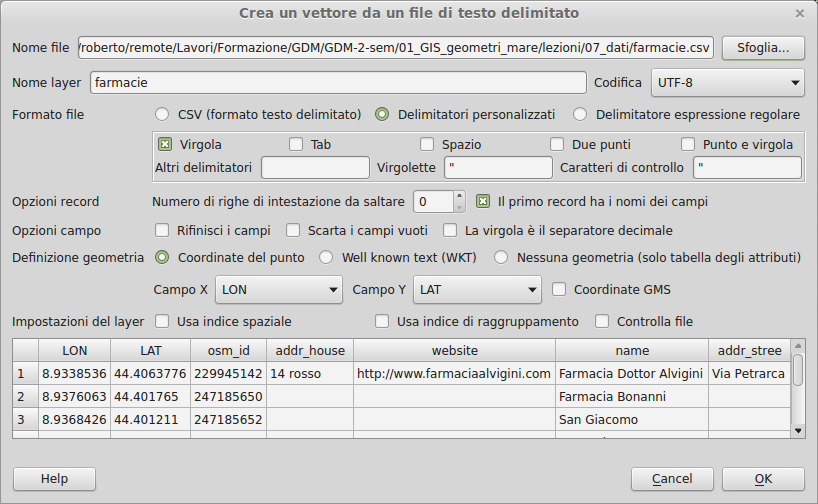
\includegraphics[width=0.8\textwidth] {digitizing_pics/import_text.png}
\end{center}
\end{frame} 


 \begin{frame}
	\frametitle{Selezioni}
	Per cancellare / modificare / unire delle geometrie bisogna utilizzare gli strumenti di selezione.
	\begin{columns}
        \begin{column}{0.5\textwidth}
            È possibile aiutarsi con le funzioni di selezione generiche
            \begin{center}
        		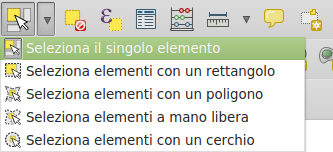
\includegraphics[width=\textwidth] {digitizing_pics/selezioni.png}
        	\end{center}
        \end{column}
        \begin{column}{0.5\textwidth}
        	o con la \texttt{selezione per espressione} (
\includegraphics[width=0.04\textwidth] {digitizing_pics/sel_exp.png})
        	\begin{center}
        		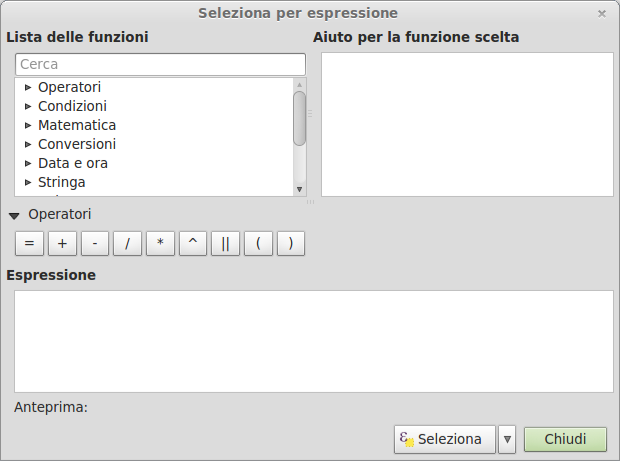
\includegraphics[width=\textwidth] {digitizing_pics/seleziona_espressione.png}
        	\end{center}
        \end{column}
	\end{columns}

\end{frame}


% \begin{frame}
%   \frametitle{Modello vettore}
%   \begin{columns}
%		\begin{column} {0.75\textwidth}	
%			Il modello vettoriale indica una rappresentazione di entità geografiche attraverso: 
%    	 \begin{itemize}
%    		\item punti,
%    		\item linee,
%    		\item poligoni.
%    	\end{itemize}
%   		I modelli vettoriali sono particolarmente utili per rappresentare e memorizzare oggetti discreti come edifici, strade, particelle, etc.					
%		\end{column}
%		\begin{column} {0.25\textwidth}	
%			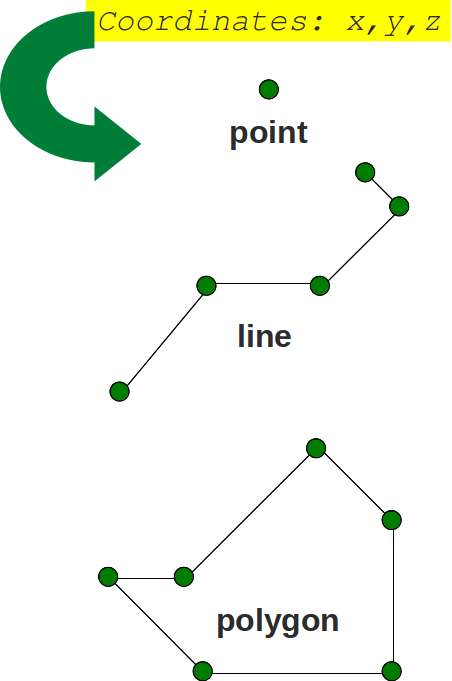
\includegraphics[width=1\textwidth] {./digitizing_pics/geom2.png}	
%		\end{column}
%	\end{columns}	
%    
%    
%   \begin{center}
%   		\textbf{Nel modello vettoriale le informazioni su oggetti discreti sono codificate ed archiviate come insieme di coordinate x,y,z}.
%   \end{center}    
%\end{frame} 


%\subsection{Importazione raster}
% \begin{frame}
%   \frametitle{Digitizing - Adding a raster layer}
%    Prepare and load the satellite imagery to QGIS. Load this raster file in QGIS by clicking \textbf{Layer} $\rightarrow$ \textbf{Add Raster Layer}.
%		    \begin{center}
%			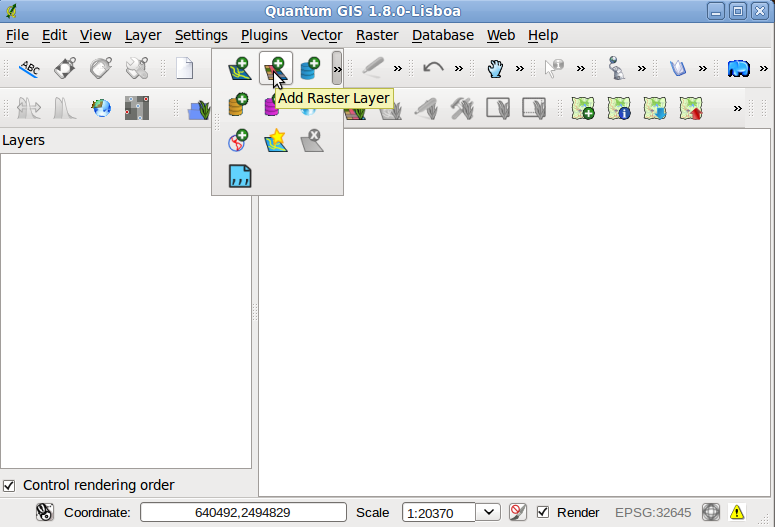
\includegraphics[width=0.80\textwidth] {digitizing_pics/add_raster.png}
%		    \end{center}
%\end{frame} 
%
%
%
%\begin{frame}
%   \frametitle{Raster properties}
%    \small To display this image to a contrast level stretch these pixels over a much smaller range. The difference between individual pixel values will be large (high-contrast) and we will see the image clearly. Go to \textbf{Style} tab. Select \textbf{Custom min/max values} and enter the value \textit{500} as the \textit{max value}. Then select \textbf{Stretch and Clip to Minmax} under Contrast Enhancement and click OK.
%		    \begin{center}
%			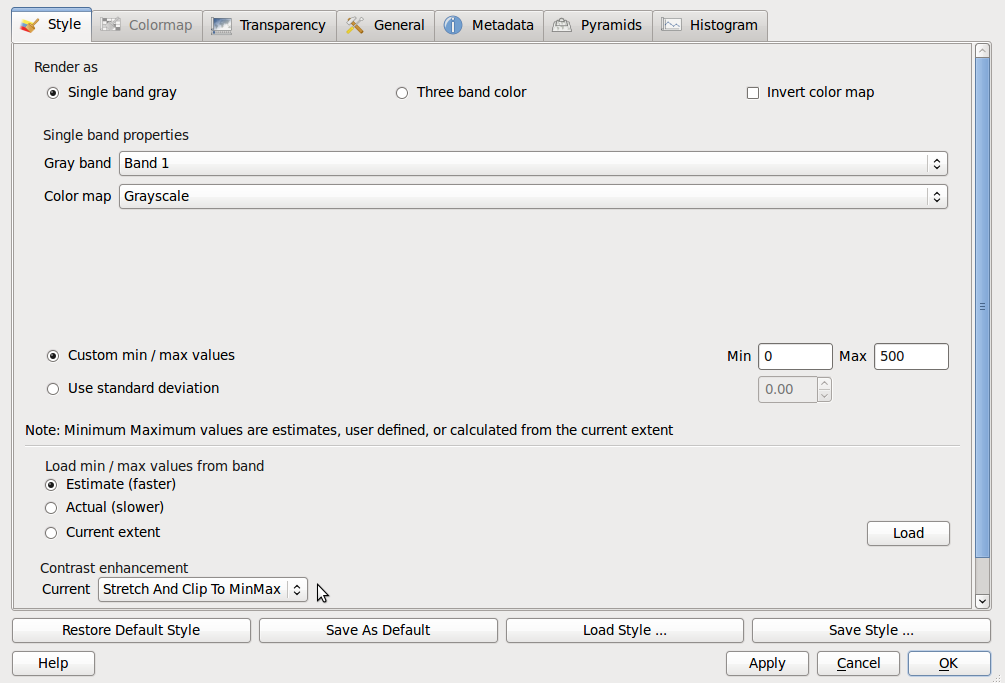
\includegraphics[width=0.60\textwidth] {digitizing_pics/contrast.png}
%		    \end{center}
%\end{frame} 
%
%
%
%
%
%
%
% \begin{frame}
%   \frametitle{Visualize raster image in grey scale}
%		    \begin{center}
%			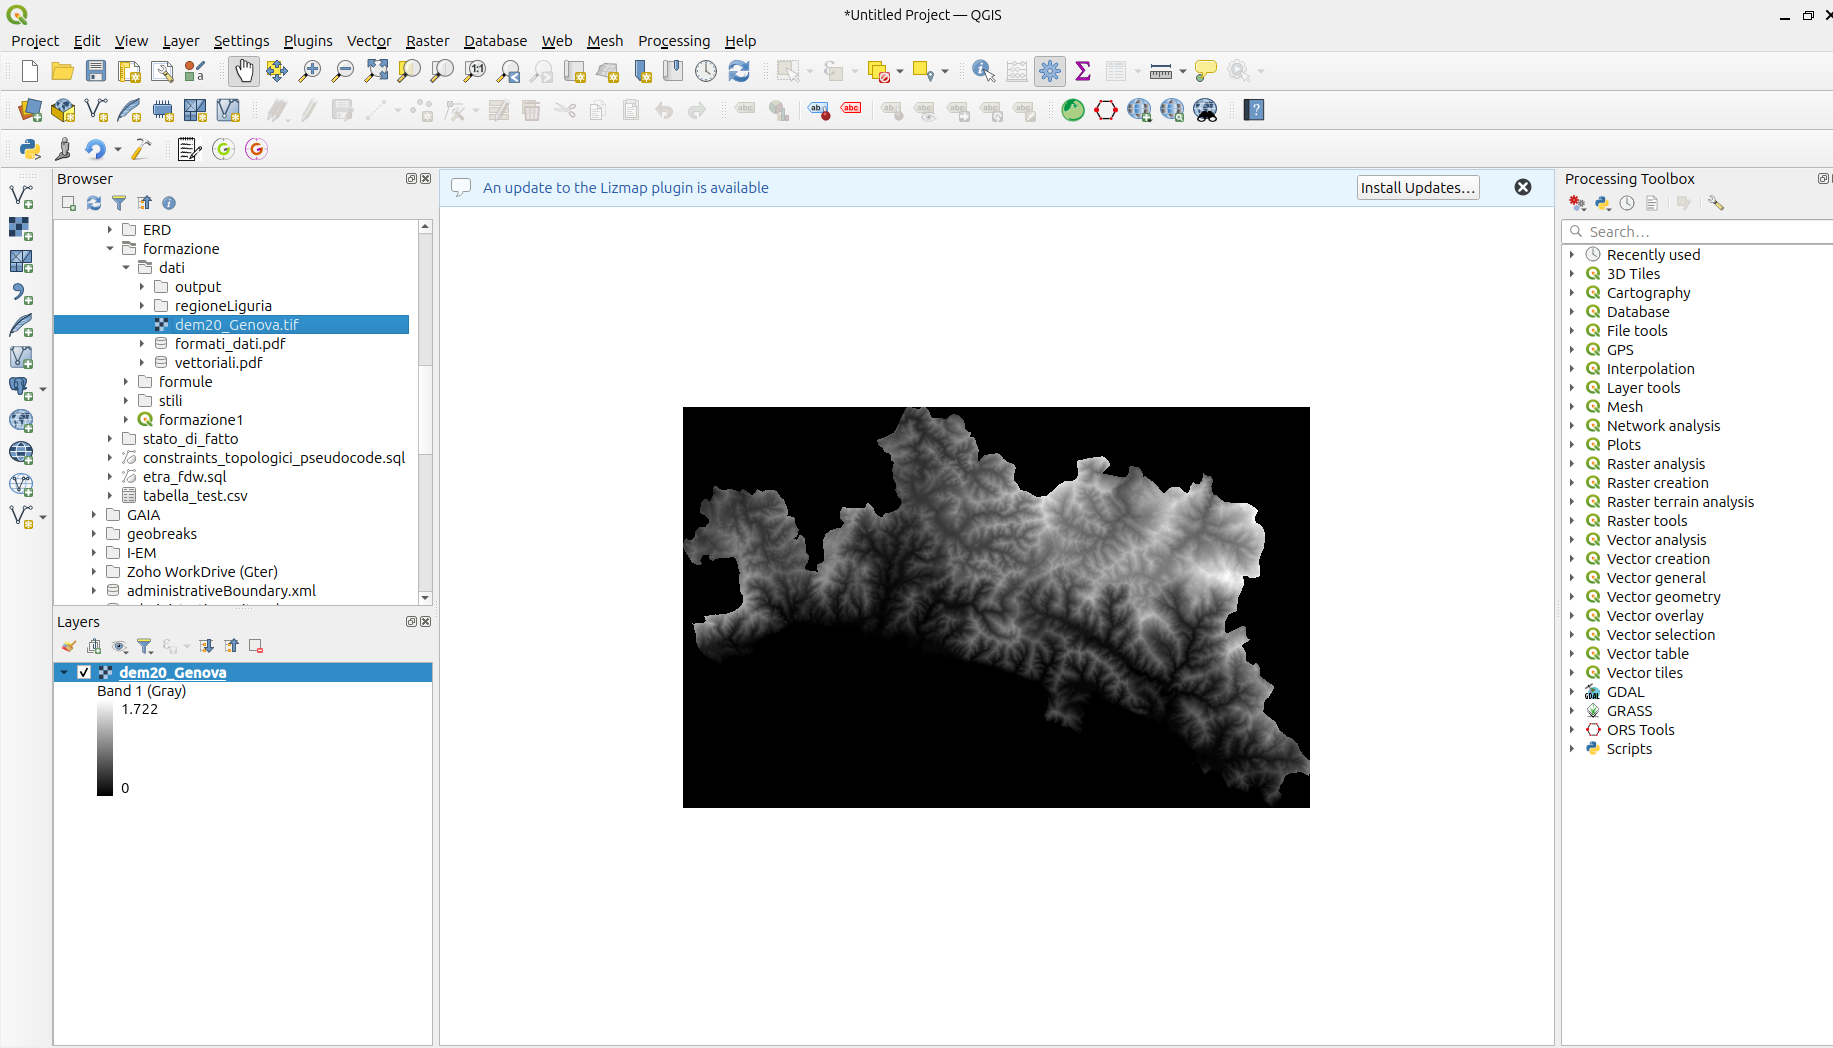
\includegraphics[width=0.90\textwidth] {digitizing_pics/grey.png}
%		    \end{center}
%\end{frame} 
%
%
%
%
%
%
%
% \begin{frame}
%   \frametitle{Set the true-color composite (3,2,1) RGB}
%    Right click on the raster layer and select \textbf{Properties}. In the \textbf{Style} tab, change the \textit{Red}, \textit{Green} and \textit{Blue} bands as it is shown below.
%		    \begin{center}
%			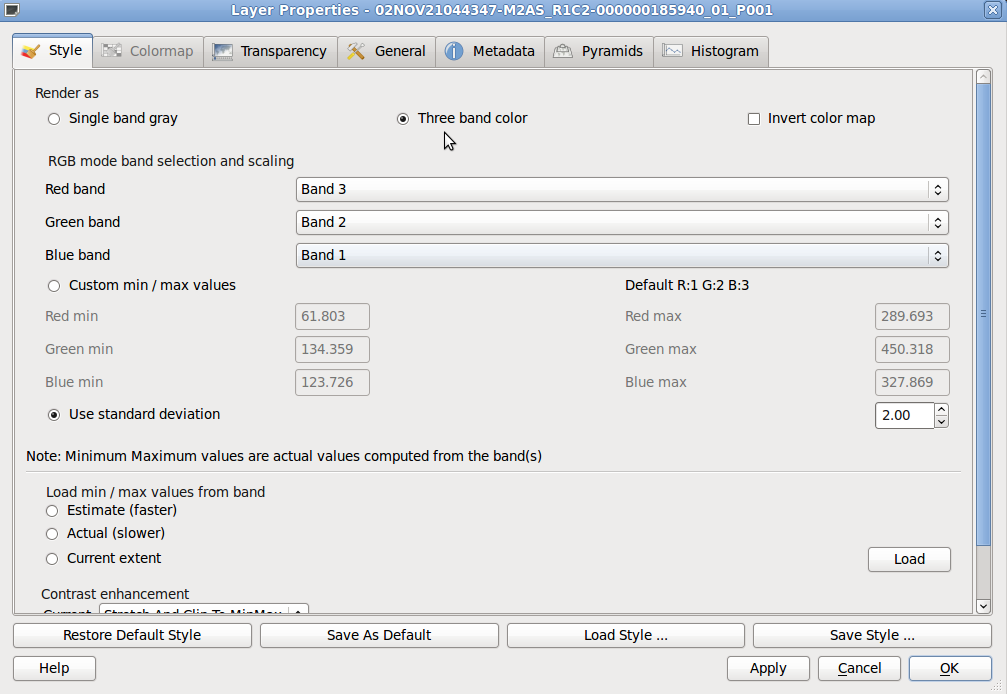
\includegraphics[width=0.82\textwidth] {digitizing_pics/321.png}
%		    \end{center}
%\end{frame}
%
%
%
%
%
%
% \begin{frame}
%   \frametitle{Visualize true-color composite (3,2,1) RGB}
%   After setting the bands in the previous step, the result looks like this..
%		    \begin{center}
%			\includegraphics[width=0.85\textwidth] {digitizing_pics/1color.png}
%		    \end{center}
%\end{frame} 

\section{Digitalizzazione}

\subsection{Creazione nuovo layer vettoriale}

\begin{frame}
    \frametitle{Creazione nuovo shapefile}
    Come \href{https://docs.qgis.org/3.22/en/docs/user_manual/managing_data_source/create_layers.html}{creare un nuovo layer vettoriale} sul quale digitalizzare punti, linee o poligoni:
    \begin{center}
        \textbf{Layer} $\rightarrow$ \textbf{Crea Vettore} $\rightarrow$ \textbf{Nuovo Layer ...}
    	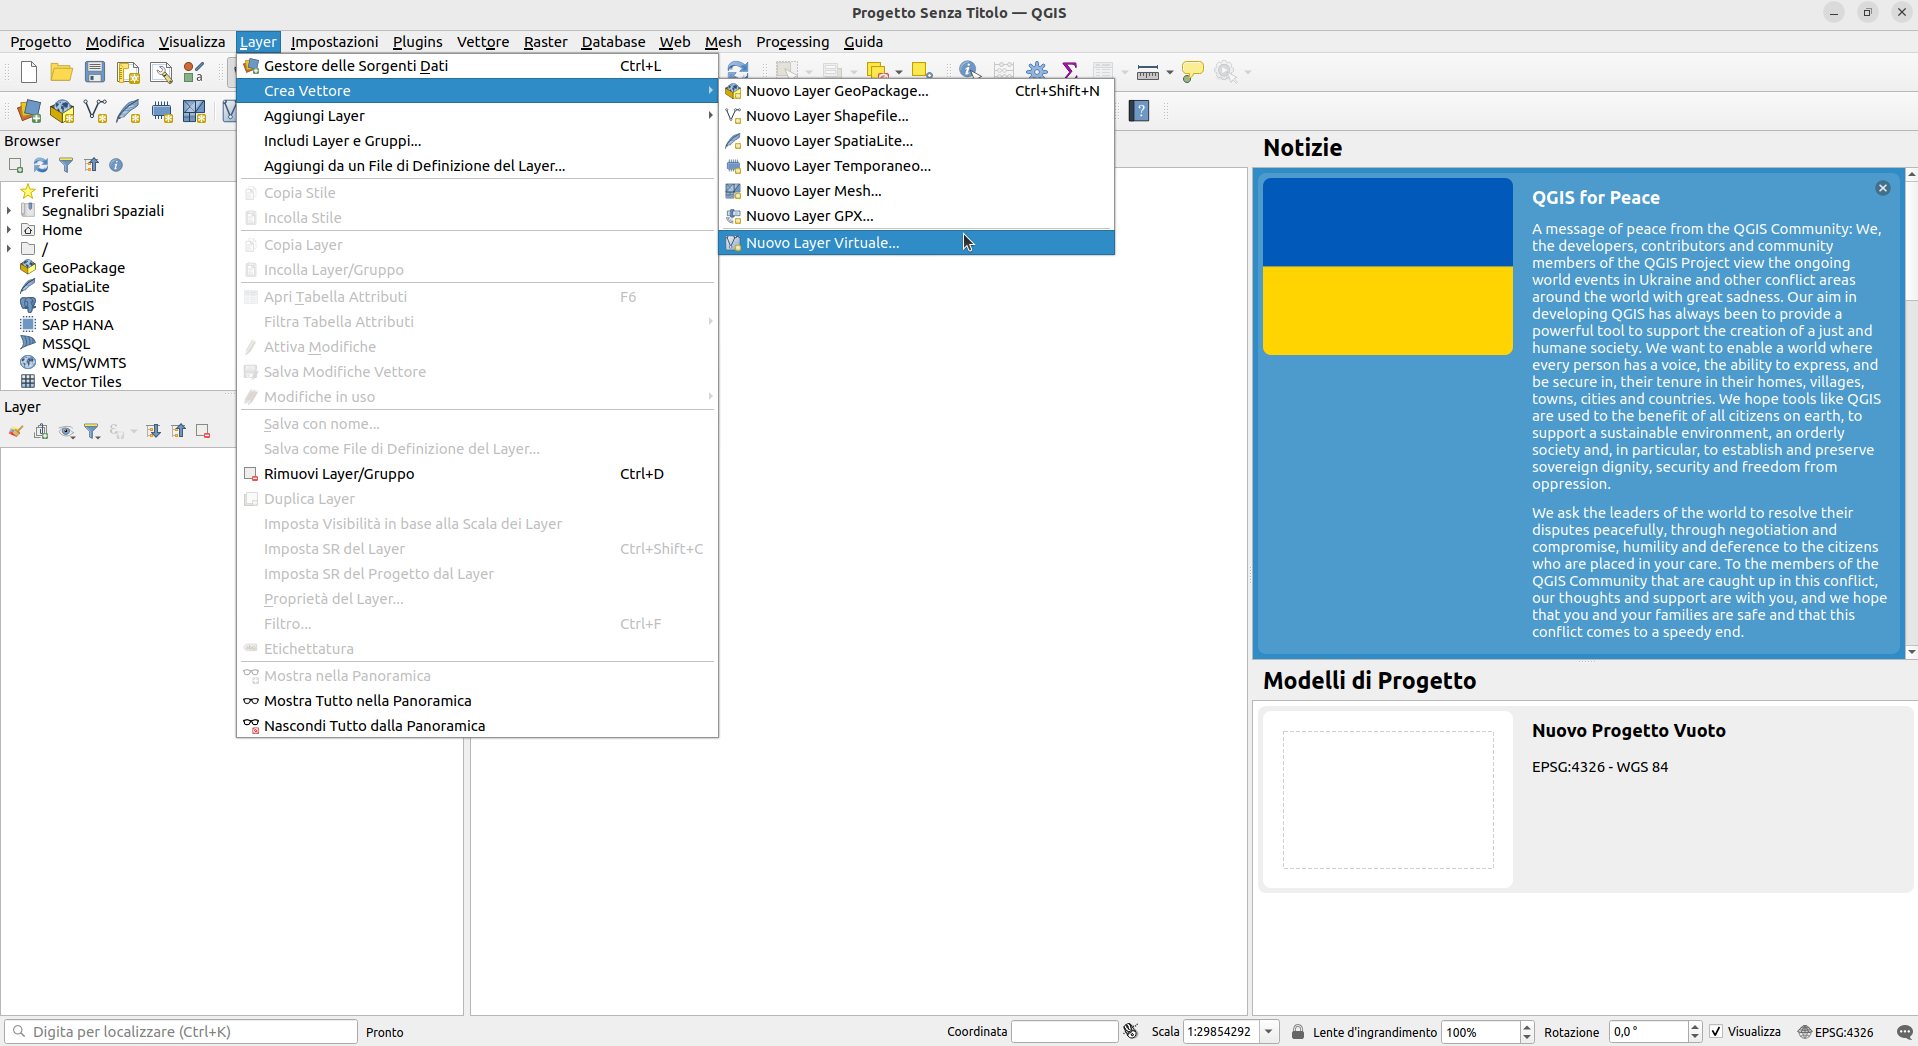
\includegraphics[width=.97\textwidth]{digitizing_pics/Nuovo vettore del 2022-10-11 09-28-13.png}
    \end{center}
\end{frame} 


 \begin{frame}
   \frametitle{Creazione di nuovo shapefile}
 	\begin{columns}
		\begin{column} {0.5\textwidth}	
			 \begin{center}
			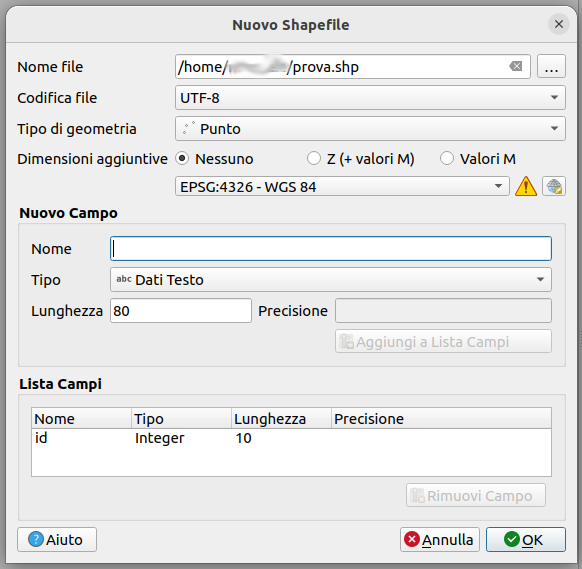
\includegraphics[width=1\textwidth] {digitizing_pics/Nuovo Layer Vettoriale 2022-10-11 09-59-20.png}
		    \end{center}
		\end{column}
 
		\begin{column} {0.5\textwidth}	
			Il settaggio del nuovo shapefile si compone di tre sezioni:  
    	 \begin{itemize}
    		\item tipologia di geometria vettoriale (punti, linee o poligoni)
    		\item SR (Sistema di riferimento),
    		\item creazione tabella degli attributi (specificare nome e tipologie dei vari campi della tabella dbf associata alla geometria vettoriale).
    	\end{itemize}				
		\end{column}
		
	\end{columns}	
	   
\end{frame} 


 \begin{frame}
    \frametitle{Scelta del SR}
    La selezione del SR associato al nuovo layer può essere fatta attraverso i codici     \href{http://www.epsg.org/}{\textcolor{gter}{\emph{EPSG}}} che li identificano in modo univoco.
    \begin{center}
        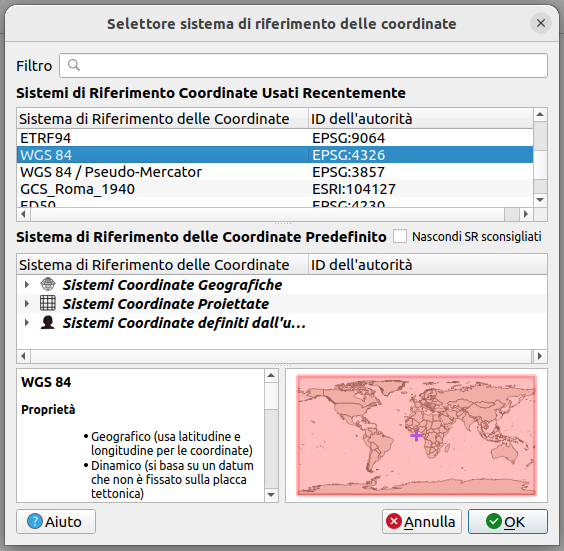
\includegraphics[height=.75\textheight] {digitizing_pics/Scelta SR.png}
    \end{center}
\end{frame} 

\section{Editing}
\subsection{Editing geometrie vettoriali}

\begin{frame}
   \frametitle{Non solo geometrie: Editing degli attributi} 
	Di default gli attributi sono tutti visti in un'unica finestra e vengono interpretati come stringhe di testo. 
	Tuttavia dalle proprietà del layer (tasto dx del mouse $\rightarrow$ Proprietà) è possibile nella finestra \textit{Campi} (o \textit{Field}):
	\begin{itemize}
		\item modificare il widget per la modifica
		\item scegliere quale modello usare per l'editor attributi: 
		\begin{itemize}
			\item \textbf{Generazione automatica}: tutti gli attributi sono presenti in un'unica finestra
			\item \textbf{Crea maschera di inserimento}: in pochi semplici passi è possibile organizzare molto bene la maschera di inserimento dati suddividendo in gruppi e sottogruppi la maschera
			\item \textbf{Fornire un file UI}: ossia fornire una maschera creata con Qt software per lo sviluppo di GUI (modalità per utenti esperti)
		\end{itemize}

	\end{itemize}
\end{frame}


\begin{frame}
   \frametitle{Editing degli attributi} 
	\begin{center}
		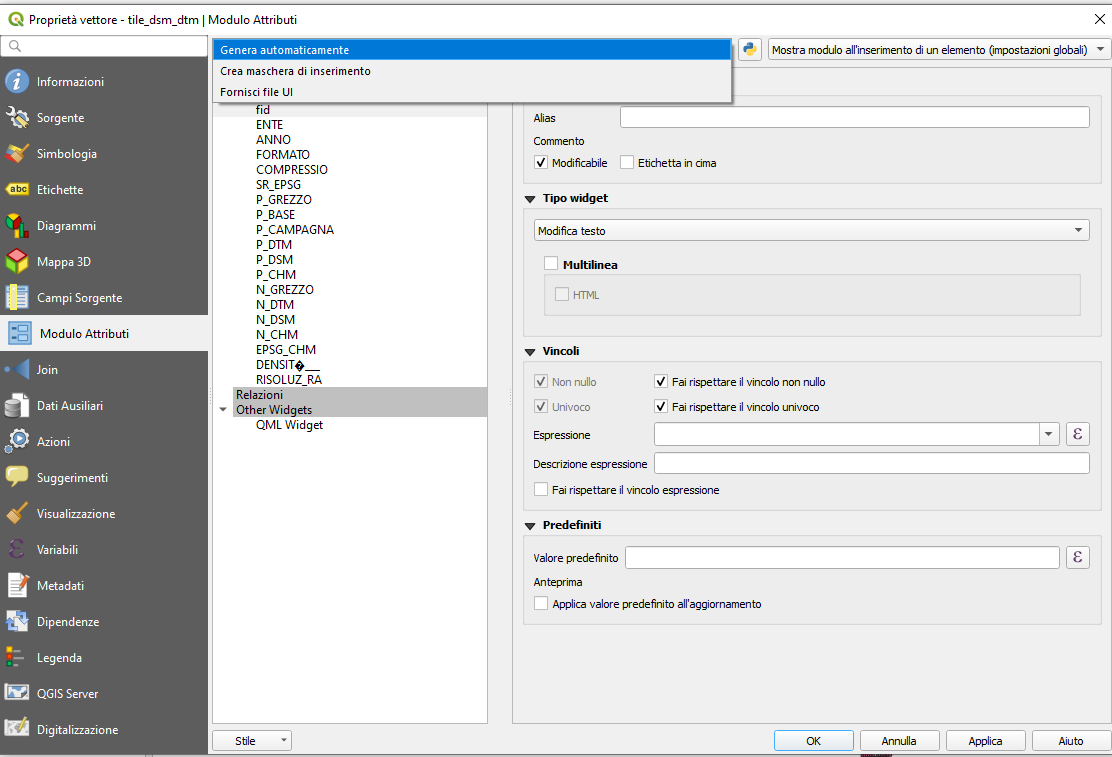
\includegraphics[width=0.9\textwidth] {pics/campi_attributi-3.png}
	\end{center}
\end{frame}


\begin{frame}
   \frametitle{Editing degli attributi} 
	Per ciascun campo si possono specificare: \begin{itemize}
		\item \textbf{alias}: nome alternativo maggiormente esemplificativo rispetto al nome della colonna
		\item \textbf{impostare un widget per la modifica}: di default casella di testo, ma volendo solo numero, percorso a un file, immagine, casella di controllo (V/F), scelta multipla (su altra tabella o su valori prefissati) 
	\end{itemize}
	\begin{center}
		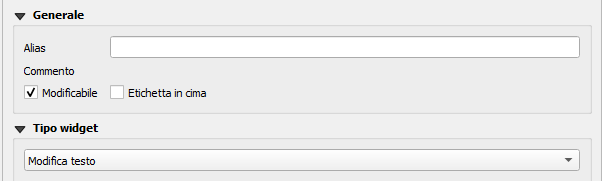
\includegraphics[width=1\textwidth] {pics/campi_attributi2-3.png}
	\end{center}
\end{frame}


\begin{frame}
   \frametitle{Attivare l'editing e gli strumenti utili}
   \begin{columns}
       \begin{column}{.5\textwidth}
            Per consentire l'\href{https://docs.qgis.org/3.22/en/docs/user_manual/working_with_vector/editing_geometry_attributes.html}{editing di un layer vettoriale}, è necessario attivare l'opzione di modifica: 
        	\begin{center}
        		 \textbf{Layer} $\rightarrow$ \textbf{Attiva Modifiche} \\
        		 oppure 
\includegraphics[height=.5 cm]{digitizing_pics/edit.png}
        	\end{center}
       \end{column}
       \begin{column}{.5\textwidth}
            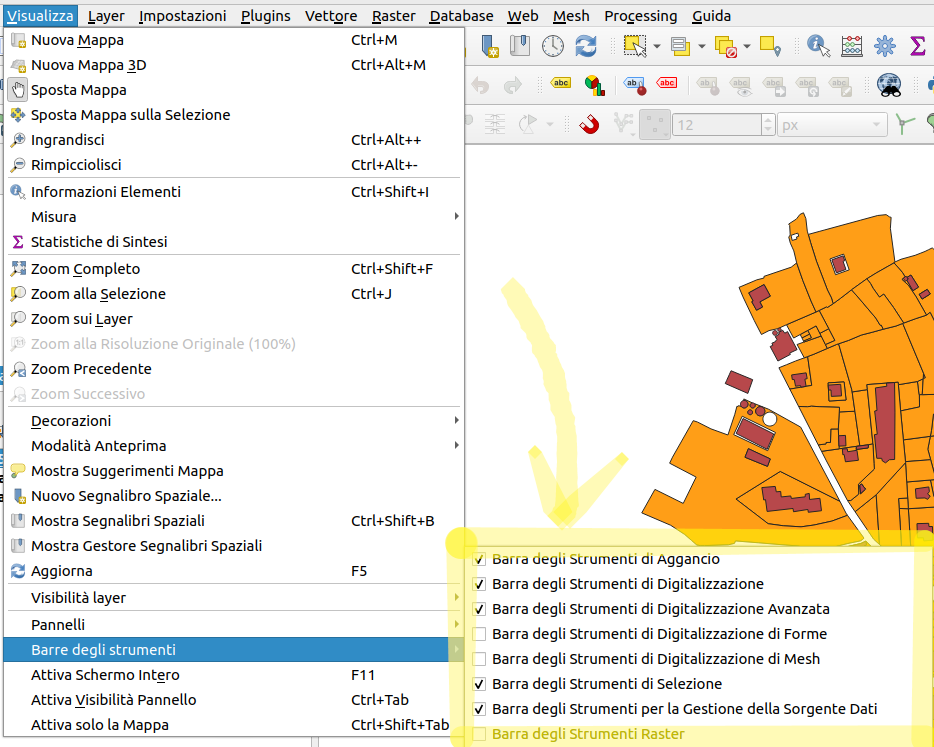
\includegraphics[width=\textwidth] {digitizing_pics/Attivazione barre strumenti del 2022-10-11 10-53-56.png}
            {\small Argomento di questa lezione:
            \begin{itemize}
                \item Strumenti di digitalizzazione
                \item ... digitalizzazione Avanzata
                \item ... digitalizzazione di forme
                \item Strumenti di Aggancio
            \end{itemize} }
       \end{column}
   \end{columns}
	
\end{frame}




%\begin{frame}
%   \frametitle{Aggiungere una nuova feature} 
%Vedi manuale:
%
%\href{https://docs.qgis.org/3.4/it/docs/user_manual/working_with_vector/editing_geometry_attributes.html#adding-features}{\textcolor{gter}{\emph{Aggiungi elemento}}}
%\end{frame}



\subsection{Modifica geometrie}

\begin{frame}
  \frametitle{Strumenti per editing di geometrie}

    \begin{columns}
        \begin{column}{.45\textwidth}
            \begin{center}
                Digitalizzazione base \\
                
\includegraphics[width=\textwidth] {pics/digit.png}
            \end{center}
            \begin{itemize}
        	 	\item attiva/disattiva modifiche
        	 	\item aggiungi geometria
        	 	\item sposta geometria
        	 	\item sposta/cancella vertici
        	 	\item elimina geometria
        	 	\item taglia/copia e incolla
        	 	\item undo/redo
        	 \end{itemize}
        \end{column}
        \begin{column}{.55\textwidth}
            \begin{center}
                Digitalizzazione avanzata \\
                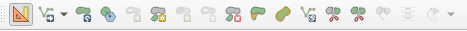
\includegraphics[width=\textwidth] {pics/digit_avanzata_barra.png}
            \end{center}
            \begin{itemize}
        	 	\item aggiungere/eliminare parti
        	 	\item unire/spezzare elementi
        	 	\item semplificazione di geometrie
        	 	\item digitalizzazione avanzata\\ \emph{stile CAD}
    	 	\end{itemize}
    	 	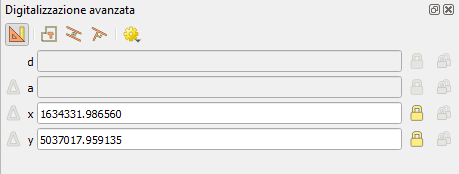
\includegraphics[width=\textwidth] {pics/digit_avanzata.png}
        \end{column}
    \end{columns}

\end{frame}

\begin{frame}{Strumenti per editing di geometrie}
    \begin{columns}
        \begin{column}{.5\textwidth}
            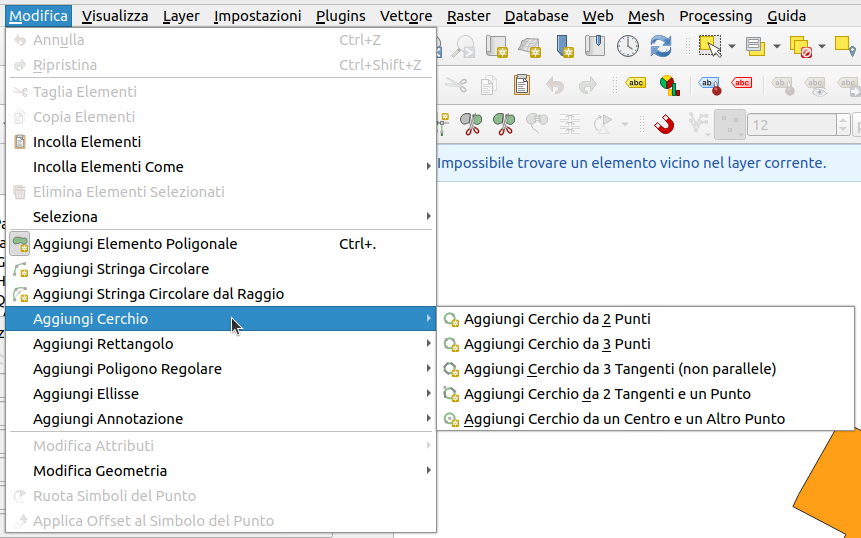
\includegraphics[width=\textwidth] {digitizing_pics/Aggiungi elementi geometrici del 2022-10-11 15-47-01.png}
        \end{column}
        \begin{column}{.5\textwidth}
            \begin{center}
                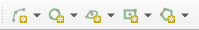
\includegraphics[width=.5\textwidth] {pics/forme.PNG}
            \end{center}
            strumenti di agevolazione per la restituzione di forme geometriche \emph{significative} secondo diversi criteri geometrici di vincolo o definizione:
            \begin{itemize}
                \item circonferenze, e archi di...
                \item poligoni regolari
                \item rettangoli
                \item ellissi
            \end{itemize}
        \end{column}
    \end{columns}
\end{frame}

%  \begin{frame}
% 	\frametitle{Strumenti di editing geometrie}
% 	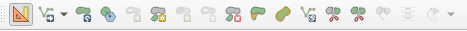
\includegraphics[width=0.4\textwidth] {pics/digit_avanzata_barra.png}
% 	 %
\includegraphics[width=0.55\textwidth] {digitizing_pics/digitalizzazione_avanzata.png}
% 	\begin{itemize}	 
% 	 \item \textcolor{blue}{\textbf{digitalizzazione avanzata}}: 
% 	 \begin{itemize}
% 	 	\item [-] digitalizzazione avanzata stile CAD
	 	
% 	 	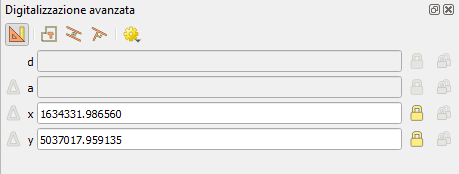
\includegraphics[width=0.4\textwidth] {pics/digit_avanzata.png}
	 	
% 	 	\item [-] aggiungere/eliminare parti
% 	 	\item [-] unire/spezzare elementi 
% 	 	\item [-] etc.
% 	 \end{itemize}
% 	 \end{itemize} 
%  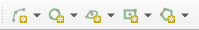
\includegraphics[width=0.4\textwidth] {pics/forme.png}
%  %
\includegraphics[width=0.55\textwidth] {digitizing_pics/digitalizzazione_avanzata.png}
%  \begin{itemize}	 
%  	\item \textcolor{gter}{\textbf{barra digitalizzazione forme geometriche}}: 
%  \end{itemize}
% \end{frame}


\section{SNAP}

\begin{frame}
   \frametitle{Snap - Strumenti di aggancio}
   Le opzioni di SNAP sono fondamentali per garantire la correttezza topologica delle informazioni 
   
		    \begin{center}
			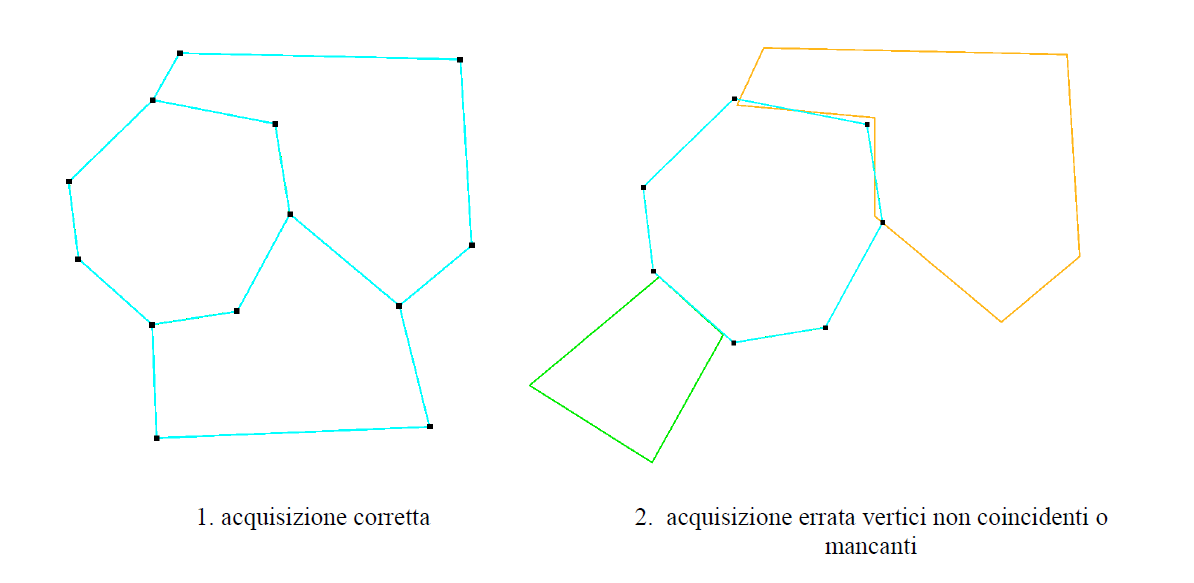
\includegraphics[width=0.90\textwidth] {digitizing_pics/correttezza.png}
		    \end{center}
    \begin{flushright}
	    \tiny{Fonte: Regione Liguria}
    \end{flushright}
\end{frame}

\subsection{Configurazione opzioni di snap}

\begin{frame}{Snap - Strumenti di aggancio: Configurazione di default}
    \begin{center}
        \textbf{Impostazioni} $\rightarrow$ \textbf{Opzioni...} $\rightarrow$ \textbf{Digitalizzazione} $\rightarrow$ \textbf{Aggancio} 
	\end{center}
    \begin{center}
        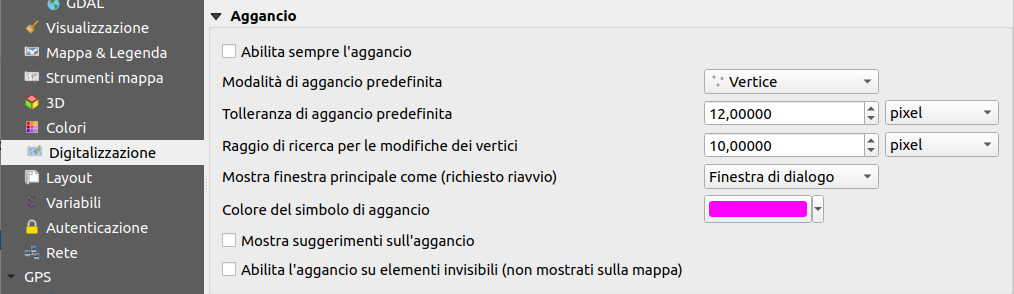
\includegraphics[width=\textwidth]{digitizing_pics/Configurazione default snap del 2022-10-12 09-27-57.png}
    \end{center}
\end{frame}

\begin{frame}
    \frametitle{Snap - Strumenti di aggancio: Attivazione e configurazione}
    Si attivano dall'apposita barra degli strumenti (
\includegraphics[width=.5 cm] {digitizing_pics/calamita.png})

    \begin{columns}
        \begin{column}{.4\textwidth}
            Opzioni di configurazione SNAP
            \begin{center}
                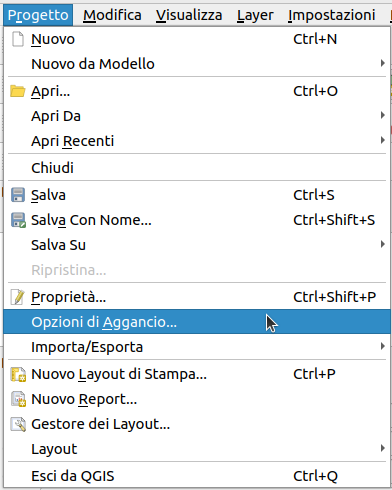
\includegraphics[width=\textwidth] {digitizing_pics/Opzioni snap del 2022-10-11 16-56-11.png}
            \end{center}
        \end{column}
        \begin{column}{.6\textwidth}
            \begin{center}
                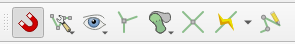
\includegraphics[width=\textwidth] {digitizing_pics/strumenti di snap del 2022-10-11 17-02-02.png}
            \end{center}
            \begin{itemize}
                \item diverse modalità
                \begin{itemize}
                    \item a tutti i layer
                    \item al layer attivo (\emph{default})
                    \item modalità avanzata
                \end{itemize}
                \item applicato a diverse geometrie
                \item con diverse tolleranze
                \item diverse unità di tolleranza
                    \begin{itemize}
                        \item $px$
                        \item unità di mappa: $m$ o $^{\circ}$
                    \end{itemize}
            \end{itemize}
        \end{column}
    \end{columns}

\end{frame}


\begin{frame}
    \frametitle{Snap - Strumenti di aggancio: Configurazione avanzata}
    Con modalità avanzata è possibile controllare la configurazione di aggancio per ogni singolo layer qualora
    \begin{center}
    	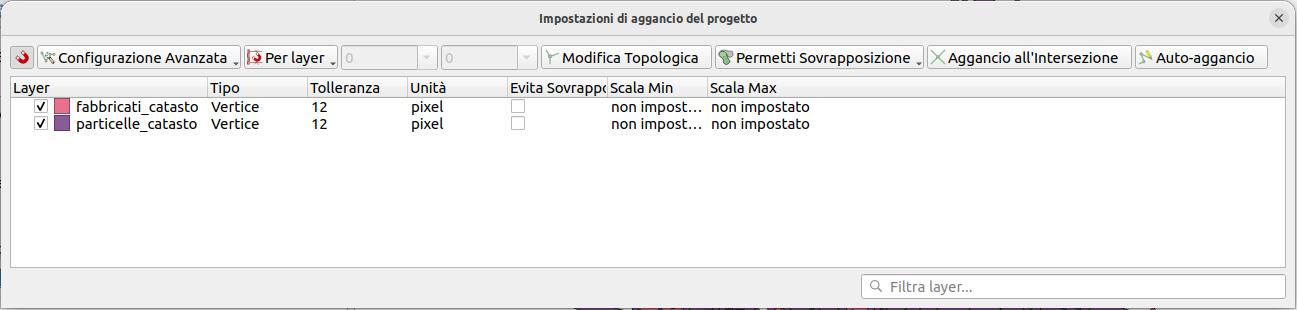
\includegraphics[width=\textwidth] {digitizing_pics/Configurazione avanzata snap del 2022-10-12 09-37-04.png}
    \end{center}
\end{frame}


\begin{frame}
    \frametitle{Snap - Strumenti di aggancio}
    \begin{itemize}
        \item \textbf{Evita intersezioni:} Regola le possibili intersezioni con altri layer poligonali evitando sovrapposizioni.
        \item \textbf{Abilita controllo topologico}: Attiva il controllo topologico con il quale si spostano insieme i vertici comuni di due elementi uniti
    \end{itemize}
\bigskip

In genere lo snap si può accoppiare alla funzionlità di aggancio (abilita ricalco) %
\includegraphics[width=0.055\textwidth] {digitizing_pics/calamita.png}) 
disponibile nelle funzionalità di digitalizzazione avanzata.
\end{frame}

\begin{frame}
   \frametitle{Considerazioni e consigli utili}

    \begin{itemize}
	    \item Fino a quando non si salva è sempre possibile annullare le operazioni precedenti una a una (undo).
	    \item Un buon consiglio è comunque quello di salvare le operazioni di editing andate a buon fine per evitare di perdere del lavoro!
	    \item Al termine dell'editing viene richiesto se salvare o meno. Non salvando tutte le modifiche effettuate dopo l'ultimo salvataggio verranno automaticamente annullate. 
    \end{itemize}
\end{frame}



 \begin{frame}
   \frametitle{Terminato l'editing}
   
		    \begin{center}
			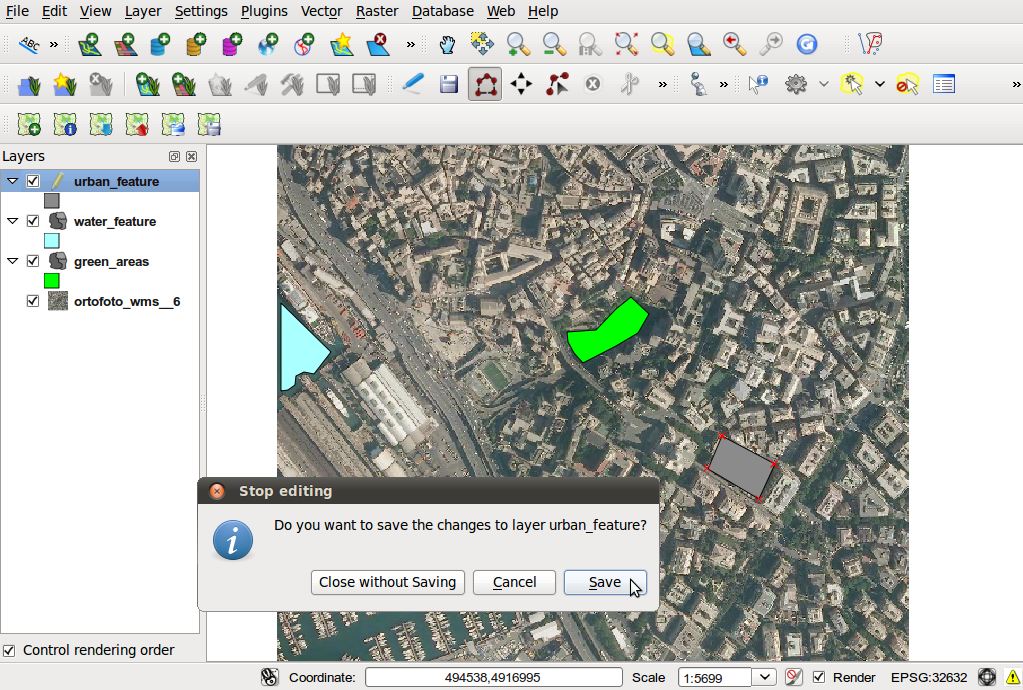
\includegraphics[width=0.95\textwidth] {digitizing_pics/finish_digit.png}
		    \end{center}

		    

\end{frame}






\section{Attributi dei layer vettoriali}

 \begin{frame}
  \frametitle{Gestione della tabella attributi}
	 \textbf{Layer} $\rightarrow$ \textbf{Apri tabella attributi}		
		
\includegraphics[height=0.4 cm] {digitizing_pics/attr.png}

		    \begin{center}
			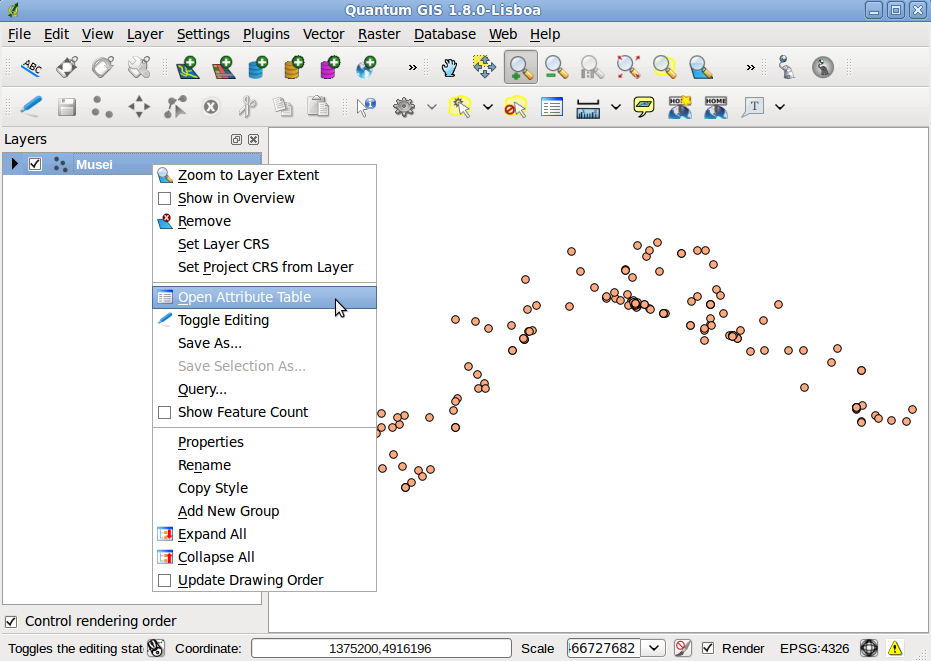
\includegraphics[width=0.80\textwidth] {topology_attrmanagement_pics/open_attr_table.png}
		    \end{center}
\end{frame}


\subsection{Query}

\begin{frame}
   \frametitle{Query}
   La tabella attributi consente di gestire la parte non geometrica dei record del layer, in particolare è possibile eseguire delle ricerche e selezionare record sulla base dei valori degli attributi.
		    \begin{center}
			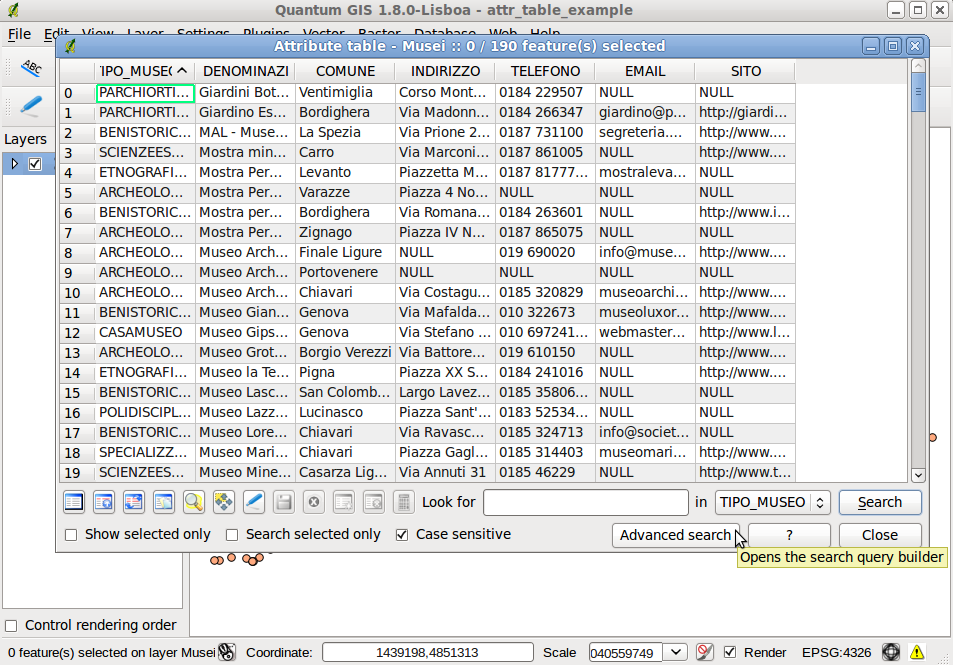
\includegraphics[width=0.80\textwidth] {topology_attrmanagement_pics/attr_table.png}
		    \end{center}
\end{frame}


 \begin{frame}
   \frametitle{Query builder}
   Si può visualizzare il query builder.
	 \begin{columns}
		\begin{column} {0.65\textwidth}	
			  \begin{center}
			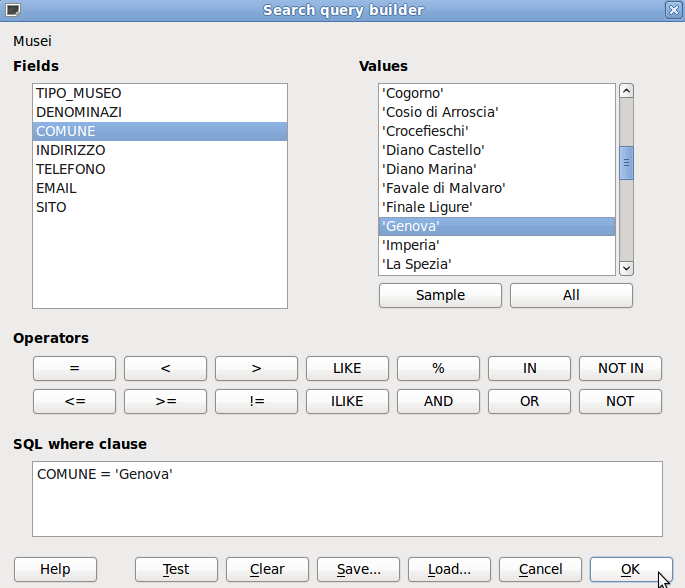
\includegraphics[width=1\textwidth] {topology_attrmanagement_pics/query.png}
		    \end{center}
		\end{column}
		
		\begin{column} {0.35\textwidth}	
  			Servendosi di: 
  			\begin{itemize}
  				\item campi
  				\item valori 
  				\item operatori
  			\end{itemize}
  			è possibile creare query anche piuttosto complesse
		  \end{column}
	  \end{columns}   
    %In the query builder window \textbf{Fields}, \textbf{Values}, \textbf{Operators} and \textbf{SQL where clauses} are shown. In this particular example, we want to highlight the museums (musei) of the town of Genova. We select: \tiny{COMUNE Fields = Genova} and click OK.
		    
\end{frame}



 \begin{frame}
   \frametitle{Risultato query}
   I record selezionati da una determinata query, come quelli dovuti ad un'eventuale selezione geometrica, risultano evidenziati nella tabella degli attributi.
		    \begin{center}
			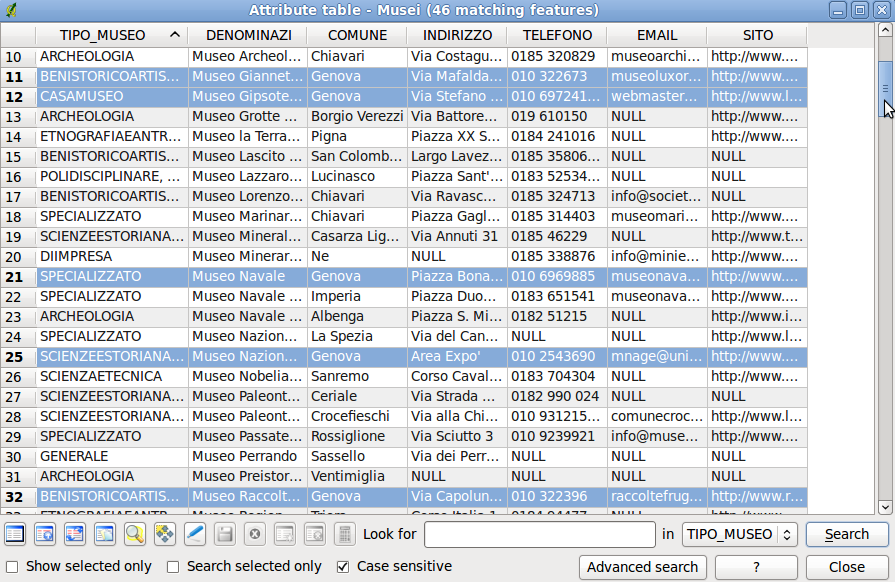
\includegraphics[width=0.80\textwidth] {topology_attrmanagement_pics/attr_query.png}
		    \end{center}
\end{frame}

 \begin{frame}
   \frametitle{Risultato query}
   ... e sulla mappa
		    \begin{center}
			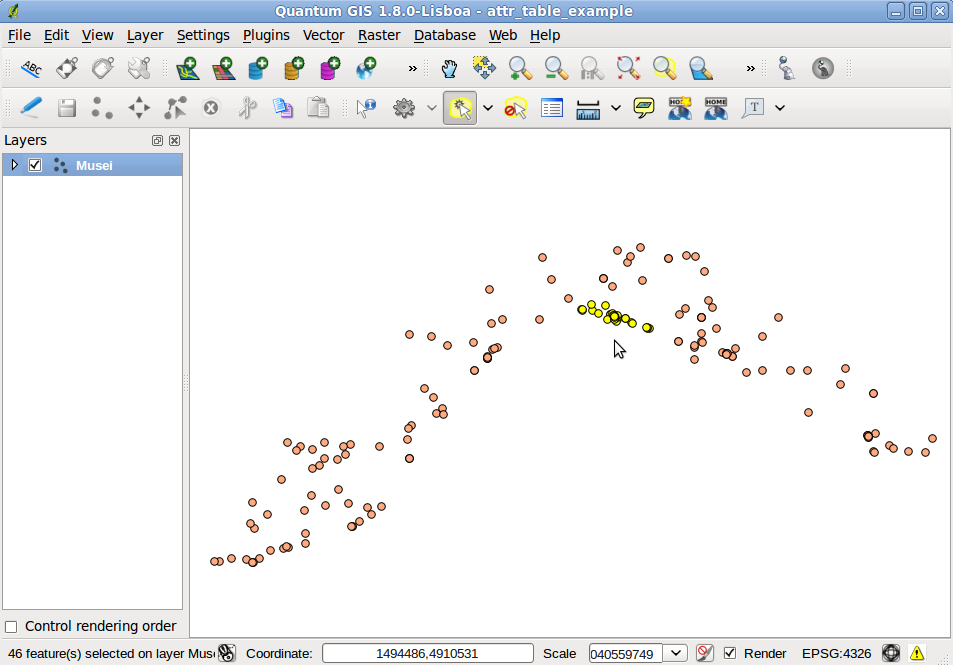
\includegraphics[width=0.70\textwidth] {topology_attrmanagement_pics/selected_qgis.png}
		    \end{center}
\end{frame}


\begin{frame}
   \frametitle{Risultato query}
   Selezionando opportunamente l'apposito flag nel riquadro in basso, è possibile visualizzare solamente i record selezionati.
		    \begin{center}
			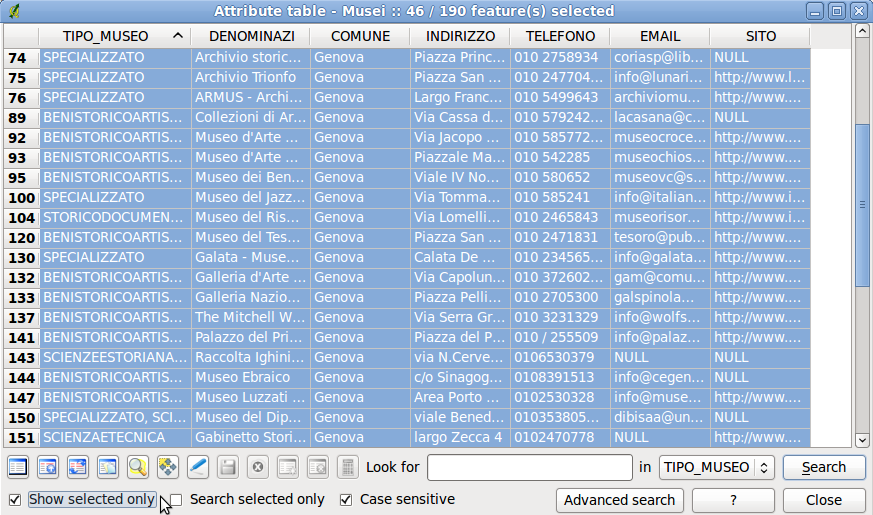
\includegraphics[width=0.80\textwidth] {topology_attrmanagement_pics/show_selected.png}
		    \end{center}
\end{frame}




 \begin{frame}
   \frametitle{Salva selezione - 1}
   Soprattutto i risultati delle query possono essere salvati in opportuni file vettoriali  \textbf{Layer} $\rightarrow$ \textbf{Salva selezione come vettore...}	
		    \begin{center}
			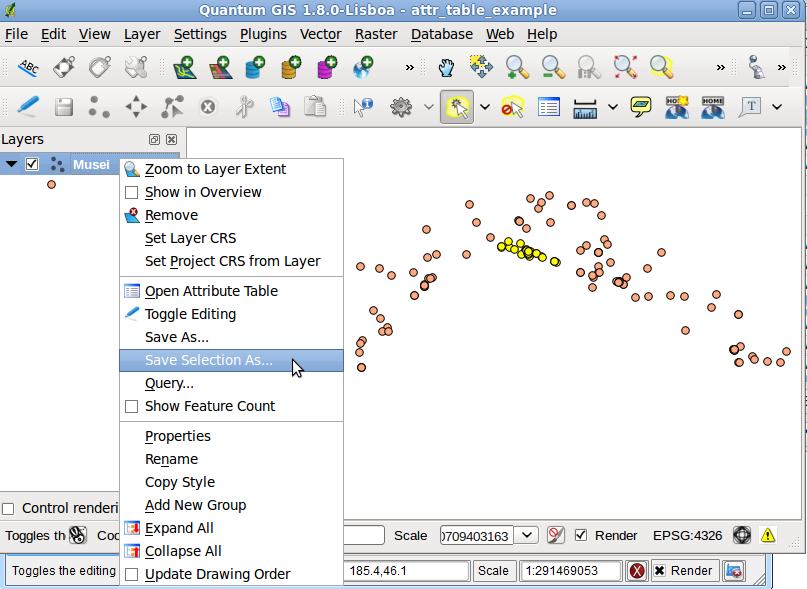
\includegraphics[width=0.70\textwidth] {topology_attrmanagement_pics/save_selection_as.png}
		    \end{center}
\end{frame}


 \begin{frame}
   \frametitle{Salva selezione - 2}
   E' possibile scegliere uno qualsivoglia fra i formati OGR: 
		    \begin{center}
			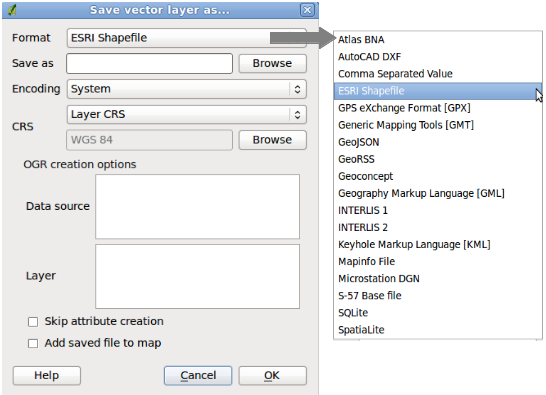
\includegraphics[width=0.75\textwidth] {topology_attrmanagement_pics/save.png}
		    \end{center}
\end{frame}


\subsection{Editing tabella attributi}
 \begin{frame}
       \frametitle{Toolbar tabella attributi - 1}
        \setbeamercolor{uppercol}{fg=white,bg=springsteen}
        Anche dalla tabella attributi è possibile attivare o disattivare le modifiche. 
\includegraphics[height=0.6 cm] {digitizing_pics/edit.png} 
              \begin{center}
		       \includegraphics[width=0.85\textwidth]{topology_attrmanagement_pics/toggle.png} 
	          \end{center}
 \end{frame}

\begin{frame}
     \frametitle{Toolbar tabella attributi - 2}
     \setbeamercolor{uppercol}{fg=white,bg=springsteen}
	 \begin{center}
	 \includegraphics[width=0.8\textwidth] {topology_attrmanagement_pics/tool_bar.png}
	  \end{center}
	\begin{itemize}
		 \item gestione selezione (inverti, deseleziona, copia etc.)
		 \item zoom mappa sulle righe selezionate
		 \item rimozione record selezionato
		 \item nuova colonna
		 \item rimozione colonna
		 \item field calculator
	\end{itemize}	 
 \end{frame}


 \begin{frame}
   \frametitle{Aggiungere una colonna}
  Trattandosi di un campo di un DB è importante specificare  \textbf{nome}, \textbf{tipo} ed eventualmente \textbf{dimensione}. 
		    \begin{center}
			\includegraphics[width=0.90\textwidth] {topology_attrmanagement_pics/add_column.png}
		    \end{center}
\end{frame}


 \begin{frame}
   \frametitle{Eliminazione colonna}
   %In order to delete an existing column of the attribute table, you only have to select the \textbf{Delete column} button and select the column you want to delete from the new window which pops up.
		    \begin{center}
			\includegraphics[width=1\textwidth] {topology_attrmanagement_pics/delete_column.png}
		    \end{center}
\end{frame}


 \begin{frame}
   \frametitle{Eliminazione feature selezionate}
   %You do the same in order to delete selected features from an attribute table. In this case you have to click on the \textbf{Delete selected features} button.
		    \begin{center}
			\includegraphics[width=1\textwidth] {topology_attrmanagement_pics/delete_selected_features.png}
		    \end{center}
\end{frame}


\section{Simbologia}
\subsection{Simbologia e rappresentazione del dato}

\begin{frame}{Simbologia e rappresentazione del dato}
    \begin{center}
        \includegraphics[width=.95\textwidth]{digitizing_pics/SImbologia del 2022-10-12 10-05-05.png}
    \end{center}
\end{frame}

\begin{frame}{Simbologia e rappresentazione del dato}
    La rappresentazione del dato ha un ruolo molto importante nella comunicazione del significato stesso che il dato porta con sé, pensiamo a come rappresenteremmo per sempio:
    \begin{itemize}
        \item aree verdi
        \item aree contaminate
        \item zone pedonali
        \item cartelli stradali
        \item ...
    \end{itemize}

    La simbologia non fa parte però delle caratteristiche o degli attributi del dato stesso, sono piuttosto attributi del progetto QGIS e sono condivisi solo concedendo l'accesso al progetto stesso.
\end{frame}


%  \begin{frame}
%   \frametitle{Field calculator - 1}
%   \begin{itemize}
%   		\item Il tool \textbf{Field calculator} \includegraphics[scale=0.55]{topology_attrmanagement_pics/fc_logo.png} permette di eseguire calcoli matematici e geometrici per modificare il valore di un campo esistente o di un nuovo campo.
%   		\item Può effettuare calcoli matematici e logici sui campi già presenti nella tabella degli attributi (es. pendenze maggiori o minori di un certo valore) o effettuare calcoli geometrici (es. calcolo lunghezze, aree, perimetri, etc.)

% 	\end{itemize}

% \small \textbf{NB} Il vettoriale deve essere abilitato per l'editing.
			
% \end{frame}




%  \begin{frame}
%   \frametitle{Field calculator}
%       \begin{columns}		
% 		\begin{column} {0.7\textwidth}
% 			\includegraphics[width=1\textwidth]{topology_attrmanagement_pics/field_calculator.png}
% 		\end{column} 	
% 		\begin{column}{0.3\textwidth}
% 		E' necessario specificare
% 		 	\begin{itemize}
% 		 		\item campo sul quale eseguire il calcolo
% 		 		\item funzioni 
% 		 		\item operatori
% %				\item \textbf{Fields list} contains all attributes of the attribute table to be searched. To add an attribute to the Field calculator expression field, double click its name in the Fields list;
% %				\item \textbf{values list} lists the values of an attribute field;
% %				\item \textbf{operators section} contains all usable operators. To add an operator to the Field calculator expression box, click the appropriate button. 
% 			\end{itemize}
% 		\end{column}
% 	\end{columns}
% \end{frame}

%  \begin{frame}
% 	\frametitle{Field calculator}
% 	\textbf{Un esempio di espressione avanzata}: supponiamo di avere un layer puntuale in un determinato SR e di voler calcolare le coordinate in un altro sistema di riferimento\\
% 	\medskip
% 	\textit{x(transform( \$geometry, 'EPSG:4326', 'EPSG:7791' ) )}
% 	\textit{y(transform( \$geometry, 'EPSG:4326', 'EPSG:7791' ) )}
% \end{frame}

%  \begin{frame}
%   \frametitle{Field calculator - measure tool}
% 	A partire dalla versione 2.0 di QGIS per effettuare le misure di aree e distanza è possibile considerare un ellissoide di riferimento
% 	\begin{itemize}
% 		\item Senza la spunta su \textit{ellissoidale} QGIS fornisce le misure piane topografiche secondo il tipo di proiezioni cartografiche  del SR (in genere UTM).
% 		\item Se si mette la spunta, si ottengono le misure riferite alla superficie curva dell'ellissoide scelto nelle \textit{Opzioni generali}.	 
% 	\end{itemize}
% Il rapporto tra distanza topografica e distanza ellissoidica è il \textit{modulo di deformazione lineare} delle proiezioni cartografiche.	
% \end{frame}

%  \begin{frame}
%   \frametitle{Field calculator - measure tool}
% 	 \begin{center}
%   \includegraphics[width=0.7\textwidth]{pics/misura.png}
%   \end{center}
% \end{frame}


%
% \begin{frame}
%   \frametitle{Join}
%	Il \textbf{JOIN} è una clausola del linguaggio SQL che serve a combinare (unire) le tuple di due o più relazioni di un database tramite l'operazione di congiunzione (o unione) dell'algebra relazionale.  
%   \begin{center}
%   \includegraphics[width=0.65\textwidth]{pics/join.png}
%   \end{center}
%\end{frame}
%
%
% \begin{frame}
%   \frametitle{Join}
%	Per utilizzare il join: tasto destro sul layer su cui effettuare il join $ \longrightarrow $  Proprietà $ \longrightarrow $ Riquadro join \\ \bigskip
%	\small Con i tasti in basso (\textcolor{gter}{\textbf{+}} / \textcolor{red}{\textbf{-}}) è possibile aggiungere o rimuovere legami con altre tabelle
%   \begin{center}
%   \includegraphics[width=0.5\textwidth]{pics/join_qgis.png}
%   \end{center}
%\end{frame}
%
%
%\section{Esercitazioni}
%
%%\begin{frame}
%%   \frametitle{Esercizio Join}
%%	Si utilizza come base dati le mappe realizzate dal \textit{\textbf{I}nventario dei \textbf{F}enomeni \textbf{F}ranosi in \textbf{I}talia} (IFFI).
%%	 \begin{center}
%%   \includegraphics[width=1\textwidth]{pics/iffi.png}
%%   \end{center}
%%\end{frame}
%
%
%% \begin{frame}
%%   \frametitle{Esercizio Join}
%%	Tale progetto ha costuito una base dati con le seguenti mappe:
%%	\begin{itemize}
%%		\item[Punti] \texttt{dati frana} (attributi tipo frana)
%%		\item[Aree] \texttt{perimetrazione\textunderscore frana} (perimetrazione)
%%		\item[Aree] \texttt{deformazioni\textunderscore gravitative\textunderscore profonde\textunderscore di\textunderscore versante} (perimetrazione)
%%		\item[Aree] \texttt{aree\textunderscore soggette\textunderscore a\textunderscore crolli\textunderscore o\textunderscore a\textunderscore frane\\ \textunderscore superficiali\textunderscore diffuse} (perimetrazione)
%%	\end{itemize}
%%
%%\begin{center}
%%Attraverso l'operazione di join filtrare le diverse tipologie di frana e ottenere come risultato le aree interessate da: 
%%\begin{itemize}
%%	\item frane superficiali diffuse;
%%	\item colamenti rapidi.
%%\end{itemize}
%%\end{center}
%%\end{frame}
%
%
% \begin{frame}
%   \frametitle{Esercizio base 1/2}
%\begin{enumerate}
%	   \item importa il file di testo con le farmacie e dati da OSM usando il plugin QuickOSM;
%%	   \\
%%	   \textcolor{red}{\textbf{Da consegnare (2-3)}}
%       \item Servendosi della foto aerea del Centro della propria città (2008), ottenuta dal WMS del PCN creare ed editare:
%       \begin{itemize}
%       		\item testare lo snap sul vettoriale delle vie
%       		\item mappa vettoriale Point of Interest (POI), usando i seguenti codici per definire i POI:
%       		 \begin{itemize}
%       		 	\item[-] 1 - Ristorante
%       		    \item[-] 2 - Bar
%       		    \item[-] 3 - Albergo
%       		    \item[-] 4 - Altro 		
%         	\end{itemize}      		 
%       		\item utilizzare la tabella \texttt{decodifica\_ POI.dbf} per creare una maschera semplificata
%       		\item creare una join con la tabella \texttt{decodifica\_ POI.dbf}	 
%       	\end{itemize} 
%       	
%		\bigskip
%		\item Creare ed editare anche le seguenti mappe:
%        \begin{itemize}      		
%        	\item mappa vettoriale delle vie (almeno 6) specificando nei campi il nome e un codice identificativo univoco
%        \end{itemize} 
%        
%      \end{enumerate}   
% \end{frame}       
%
% \begin{frame}
%   \frametitle{Esercizi 2/2}        
% \begin{itemize} 
%       \item Servendosi delle funzioni del field calculator valutare coordinate dei punti (! specificare nel nome del campo il sistema di coordinate utilizzato), lunghezza delle vie editate (geometry functions).
%   
%       %\item Provare alcune query e/o selezioni in funzione p.es. dell'area o della lunghezza 
%\end{itemize}         
%      
%\end{frame}


%\begin{frame}
%   \frametitle{Consegna}
% 	Da consegnare: 
% 	\begin{itemize}
% 		\item sintetica relazione in formato PDF dell'esercizio svolto che spieghi: 
% 		\begin{itemize}
% 		\item[-] lo scopo dell'esercizio illustrando quali sono  i dati i input a disposizione;
% 		\item[-] i vari passaggi svolti per raggiungere l'obiettivo a partire dai dati di input;
% 		\item[-] i risultati ottenuti e gli allegati alla consegna (file di output richiesti). 
% 		\end{itemize}
% 		\item file di output in formato \textit{ESRI shapefile}. 
% 	\end{itemize}
% 	\bigskip
% 	Quando?\\
% 	La prossima settimana a lezione o via mail entro il 14 maggio 2016. 
%
%\end{frame}



}
\subsection{Contatti e licenze}
{
\setbeamertemplate{footline}{} 
\setbeamertemplate{headine}{} 
\frame{	
\addtocounter{framenumber}{-1}  % non conto questa slide
\begin{center}
\bigskip
\includegraphics[width=0.2\textwidth]{./Gter.png} \\ 
\scriptsize{
%Gter srl Innovazione in Geomatica Gnss e Gis\\
Piazza De Marini 3/61\\
16123 Genova\\
formazione@gter.it\\}
\normalsize
\bigskip
\href{www.gter.it}{\textcolor{gter}{\emph{www.gter.it}}}
	
\bigskip	

  	\href{https://twitter.com/@gteronline} { \includegraphics[width=0.15\textwidth]{./tw.jpg}}
	\hspace{30pt}
	 \href{http://www.facebook.com/Gteronline} { \includegraphics[width=0.15\textwidth]{./fb.jpg}}
		\hspace{30pt}
%	 \href{ https://plus.google.com/+GterIt/posts} { \includegraphics[width=0.15\textwidth]{../go.png}}
%	 \hspace{30pt}
	 \href{http://www.linkedin.com/company/gter-srl-innovazione-in-geomatica-gnss-e-gis} { \includegraphics[width=0.15\textwidth]{./ln.png}}
	 
	 
	 

	 
\bigskip
\vspace{30pt}

	
	\href{http://creativecommons.org/licenses/by-sa/3.0/deed.it} {	
	\includegraphics[width=0.15\textwidth]{./88x31.png} 
	\\	
	\tiny Quest' opera è distribuita con licenza Creative Commons Attribuzione - Condividi allo stesso modo 3.0 Unported.} 	
	
	
	
\end{center}
%\tableofcontents[pausesections,part=2]
}
}

\end{document}
